%Group Report Information: Did it work properly? What kind of tests did you run to test your prototype? Could you provide some data that shows the performance of the prototype (speed, success rate, etc.)?

\section{Results/Analysis}
We originally believed that we could somehow calculate the length between MR and ML. This mistake only came up when we began to program the software part after having produced much of the prototype. The solution was to assume a fixed length between MR and ML. The results are also skewed as a result of the magnets for homing (endstop) not being close enough to the end of the wire. This causes an incorrect measurement of line width. This is quite noticeable on figure \ref{SkewedDrawing} where the supposed circle becomes an oval. This is a problem with accuracy as the machine keeps hitting the same place when it wants to reach a coordinate, but it is not always the correct coordinate. Therefore, our drawing machine has reached a medium accuracy and a higher precision (medium because it is clearly still high enough that one can make out what it is drawing in most cases, exceptions being that circles becomes ovals etc.).\\
% Another source of error, and this is mainly on the basis of suspicion is that one motor
Notice that the text suddenly jumped, this was due to the heatsink having fallen off the Pololu a4988 driver (thus overheating and the driver shutting down for protection).

\begin{figure}[h]
\centering
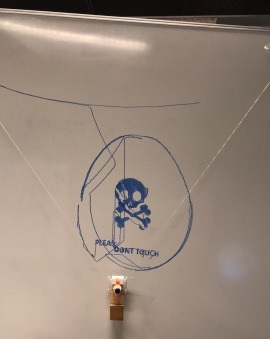
\includegraphics[scale=0.60]{Images/DrawingMachine/SkewedDrawing.jpg}
\caption{ Drawing machine skewed drawing. }
\label{SkewedDrawing}
\end{figure}